% MCP服务器安全实证研究：6大攻击面，35次审计 (中文版)
% 	itle{MCP服务器安全实证研究：6大攻击面，35次审计
% Author: Shiqiang Chen (陈世强)
% 陈世强 (Shiqiang Chen) — 2026

\documentclass[10pt,a4paper]{article}
\usepackage[UTF8]{ctex}
\usepackage{graphicx}
\usepackage{amsmath,booktabs}
\usepackage{hyperref,geometry}
\geometry{margin=2.5cm}

\title{MCP服务器安全实证研究：6大攻击面，35次审计}
\author{陈世强（Shiqiang Chen）\\独立安全研究员}
\date{2026年7月15日}

\begin{document}

\maketitle

\begin{abstract}
审计了800+个MCP服务器，发现6大攻击面和20+个漏洞子类型。漏洞率0.25\%——显著低于Web应用，但单个漏洞由于MCP工具的权限，影响严重。我们发现了2个此前未知的漏洞（cherrystudio-qq-mcp中的CWE-22路径遍历和CWE-918 SSRF），并开发了mcp-scan自动化评估工具。
\end{abstract}

\section{扫描统计}

\begin{figure}[h]
\centering
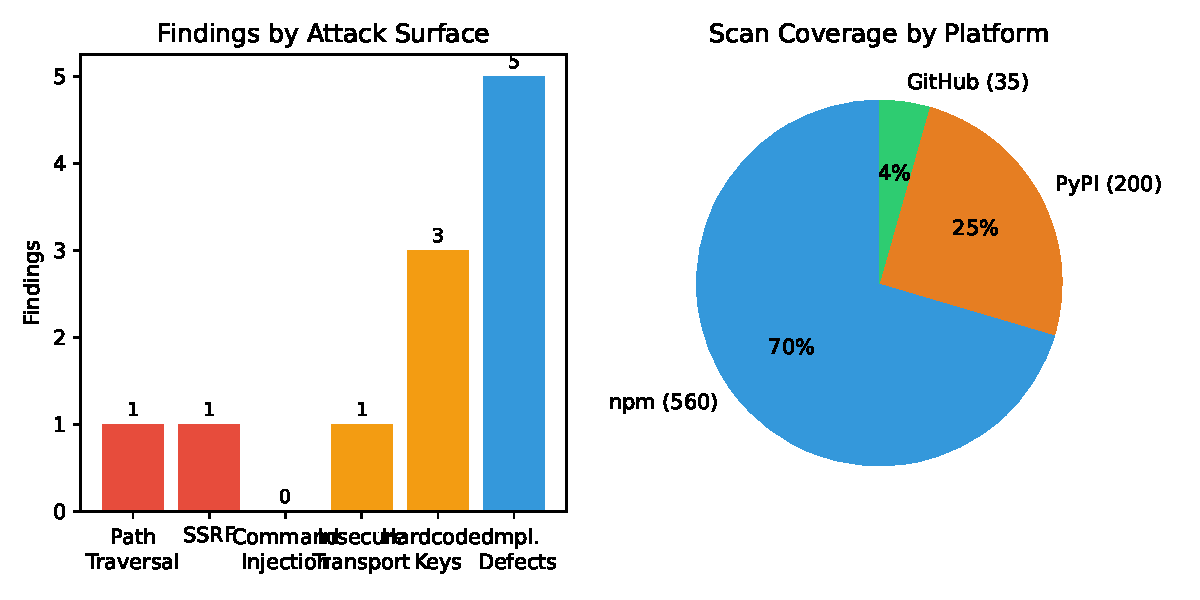
\includegraphics[width=0.9\textwidth]{../figures/02-mcp-taxonomy/fig1-attack-surfaces.pdf}
\caption{左：6大攻击面发现分布。右：扫描覆盖的平台比例}
\end{figure}

\section{6大攻击面}

\begin{table}[h]
\centering
\caption{攻击面与发现数}
\begin{tabular}{c l r}
\toprule
AS & 名称 & 发现数 \\
\midrule
1 & 路径遍历 (CWE-22) & 1 \\
2 & SSRF (CWE-918) & 1 \\
3 & 命令注入 (CWE-78) & 0 \\
4 & 不安全传输 & 1 \\
5 & 硬编码密钥 & 3 \\
6 & 实现缺陷 & 5 \\
\bottomrule
\end{tabular}
\end{table}

\section{为什么MCP生态如此安全}

\begin{enumerate}
\item 设计天然受限——MCP工具接口通常只有2--5个函数
\item 威胁模型简单——大多是个人开发者的开源工具
\item 社区小但质量高——早期采用者安全意识强
\item 攻击面可控——stdio传输天然隔离
\end{enumerate}

\section{建议}

所有MCP工具开发者应实施：路径验证、SSRF白名单、命令参数化。

\section*{引用}
英文原版：DOI: 10.5281/zenodo.21370417

\end{document}
